% LaTeX-Vorlage für Dokumente an der IBS
% nur für kurze Ausarbeitungen

% #################################################################################
% Header
% #################################################################################
\documentclass{scrartcl}						% Basisdokumentenklasse
\usepackage[ngerman]{babel}        	% Deutsche Standardbezeichner und Trennung
\usepackage[utf8]{inputenc}     		% Für Umlaute; dabei auf Kodierung des Editor achten
\usepackage[T1]{fontenc}           	% und ß
\usepackage{abstract} 							% Für Abstracts
\usepackage{float}
\usepackage[hyphens]{url}
\usepackage{nohyperref}
\usepackage{amsmath}
\usepackage{float}
\usepackage{enumitem}
% #################################################################################

\usepackage{ibs}										%Immer zuletzt einbinden

% #################################################################################
% Das eigentliche Dokument
% #################################################################################
\begin{document}

%Titel
\title{Situationsanalyse und Marketing Mix}
\author{Jens Kessen, Timon Menke, Jameel Hassan, Jan Budde}

\publishers{Begutachtende: Dr. Birte Janssen}
\maketitle %dadurch wird der Titel auch erstellt

\renewcommand{\abstractname}{Abstract} %so heißt es auch "Abstract"; Voreinstellung ist "Zusammenfassung"
\thispagestyle{empty}
%Abstract

%\begin{center}
%\begin{abstract}
%\noindent %Die erste Zeile des Abstrakts soll nicht eingrückt werden

%\end{abstract}
%\end{center}

\pagebreak
\tableofcontents %damit kann ein Inhaltsverzeichnis eingefügt werden
\pagebreak

% Fußzeilen ab Seite 1 (fancy style auch auf titelpage)
\thispagestyle{fancy}

% Inhalte einfügen
\newcommand{\as}{\glqq}
\newcommand{\ad}{\grqq}
\newcommand{\adl}{\grqq{ }}

\newcommand{\fref}[1]{Abb. \ref{#1}} %Ref Figures

\section{Situationsanalyse} \label{sitana}
    

\subsection{Persona B} \label{personaB}
    Bei unserer zweiten Persona handelt es sich um Andreas Martens. Andreas ist 40 Jahre alt, verheiratet und hat zwei 
    Kinder. Er interressiert sich für unser Produkt, da er es sehr gut für seine Arbeit in der Gebäudepflege, welche er 
    seit 20 Jahren ausübt, einsetzen kann. Außerdem ist er sehr Technikbegeistert und ist auf der Suche nach 
    alternativen Arbeitswegen, mit welchen er sich seine Arbeit erleichtern und die Sicherheit erhöhen kann. Ebenfalls 
    ist er auf der Suche nach mehr Effizienz und nach einem Zuverlässigen Produkt.

    Über neue technologische Entwicklungen informiert er sich vor allem über Fachmagazine, wie zum Beispiel \as Der
    Hausmeister\adl, oder auch über das Radio.

\subsection{SWOT-Analyse} \label{swot}
Um nun externe und interne Informationsbereiche miteinander zu verbinden, wird die \as SWOT-Analyse\adl genutzt. Mit
dieser Betrachtung ist es möglich, die Stärken und Schwächen des Unternehmens kombiniert mit den Chancen und Risiken der
Mikro- und Makroumwelt zu untersuchen und Strategien abzuleiten.


\section{Marketing Mix} \label{Mix}


\subsection{Kommunikationspolitik} \label
    Nachdem nun die Produktpolitik betrachtet wurde, folgt die Kommunikationspolitik. Dieses Werkzeug des 
    Marketing-Mixes beschreibt die Wege, mit denen das Unternehmen mit seinen Kunden in Kontakt tritt und diese mit
    Informationen und Werbung versorgt. (Vgl. \cite{Kuss2016} S.\,203)

    \noindent
    Bei der Entwicklung der Kommunikationspolitik ist die Auswahl der Marketingträger und -plattformen von essenzieller
    Bedeutung. Um die wirkungsvollsten Träger auszuwählen, müssen zunächst wieder die Personas aus der Situationsanalyse
    betrachtet werden. Danach werden für diese Zielgruppen entsprechende Kommunikationswege gewählt.

    \noindent Im Fall \as RinnenRobo\adl gibt es die folgeden zwei Zielgruppen:

    \begin{enumerate}
        \item Hauseigentümer, vor allem ältere Personen
        \item Dienstleister in der Gebäudepflege
    \end{enumerate}

    \noindent Um für diese Zielgruppen nun die Kommunikationsmedien zu wählen, wird mit der Intermediaselektion begonnen.
    
    \noindent Für die erste Zielgruppe wurden folgende Medien herausgestellt:

        \begin{itemize}
            \item Fernsehen
            \item Radio
            \item Zeitung
        \end{itemize}

    \noindent Um die Dienstleister zu erreichen, wurden die folgenden Medien gewählt: 

        \begin{itemize}
            \item Fachmessen
            \item Fachmagazine
            \item Direktmarketing
        \end{itemize}

    \noindent
    Bei der Auswahl dieser Medien wurde betrachtet, auf welchen Medien die Personen der entsprechenden Zielgruppe häufig
    anzutreffen sind. Somit wären hier auch die Chancen für eine erfolgreiche Marketingkampagne hoch.

    \noindent
    Im nächsten Schritt werden die einzelnen Kommunikationskanäle genauer betrachtet und es findet die
    Intramediaselektion statt. Hierbei werden konkrete Möglichkeiten innerhalb der Plattformen herausgearbeitet. Dabei
    wird wieder versucht, die Teilkanäle zu wählen, bei denen ein Antreffen von potenziellen Kunden am
    wahrscheinlichsten ist.

    \noindent
    Die Intramediaselektion für die Gruppe der Hauseigentümer sieht folgendermaßen aus:

    \begin{itemize}
        \item Fernsehen
            \subitem Das Erste
            \subitem ZDF
            \subitem NDR
        \item Radio
            \subitem NDR 1
            \subitem Bremen 1
        \item Zeitung
            \subitem Lokale Tageszeitung
    \end{itemize}

    \noindent
    Für die Dienstleister wurden folgende Teilkanäle gewählt:

     \begin{itemize}
        \item Messen
            \subitem IPM Essen
            \subitem GaLaBau
            \subitem CMS Messe Berlin
        
        \item Fachmagazine
            \subitem Der Hausmeister
            \subitem Galabau Journal

        \item Direktmarketing
            \subitem Prospekte
            \subitem Flyer
     \end{itemize}

    \noindent
    Auf den genannten Teilkanälen wäre also eine Kommunikation mit Personen der entsprechenden Zielgruppe möglich.

    \noindent
    Um nun konkrete Marketingmaßnahmen planen und durchführen zu können, muss außerdem eine Budgetstrategie festgelegt
    werden. Diese Strategie besagt, wie viel Kapital für die Kommunikationspolitik ausgegeben werden darf. Dieses
    Kapital wird beispielsweise für Fernsehspots oder Werbeanzeigen in der lokalen Tageszeitung benötigt.
    (Vgl. \cite{Bruhn2014a}, S.\,212)

    \noindent
    Es gibt sowohl analytische als auch heuristische Verfahren zur Budgetierung. Bei den analytischen Ansätzen wird das
    verfügbare Kapital durch mathematische Funktionen errechnet, während dieses bei heuristischen Ansätzen nach
    vereinfachten Regeln festgelegt wird (vgl. \cite{Bruhn2014a}, S.\,214).

    \noindent
    Im Folgenden werden jedoch nur die heuristischen Ansätze weiter betrachtet.

    \noindent
    Diese heuristischen Verfahren lassen sich in drei weitere Untergruppen gliedern. Diese werden im Folgenden genannt
    und näher erläutert.

    \begin{itemize}
        \item Unternehmensbezogene Ansätze
            
            Bei dieser Art von Budgetierung werden unternehmensinterne Werte zur Budgetkalkulation herangezogen. So kann
            beispielsweise ein gewisser Prozentsatz des Umsatzes für Kommunikationsmaßnahmen eingesetzt werden.

        \item Konkurrenzbezogene Ansätze
        
            Hier orientiert sich ein Unternehmen an den Werbebudget und -ausgaben der Konkurrenz und versucht auf dessen
            Grundlage die eigene Marketingbudgetierung vorzunehmen.

        \item Marktbezogene Ansätze
        
            Bei diesen Ansätzen liegt der Fokus auf dem zu erreichenden Ziel. Daraus wird das benötigte Budget bestimmt.
            So kann das Ziel etwa eine Bekanntheit von 20\% auf dem deutschen Markt sein. Hieraus wird nun das zum
            Erreichen dieses Ziels benötigte Budget bestimmt.
    \end{itemize} (Vgl. \cite{Bruhn2014a}, S.\,214)

    \noindent
    Im Praxisbeispiel \as RinnenRobo\adl wird ein unternehmensbezogener Ansatz genutzt. Genauer: Es soll so viel
    Kapital für die Durchführung der Marketingmaßnahmen genutzt werden, wie verfügbar ist.

    \noindent
    Diese Entscheidung ist begründet durch das allgemeine Unwissen über die Existenz von Rinnenreinigungsrobotern und
    den Wunsch \as RinnenRobo\adl zu einer bekannten Marke zu entwickeln, um auch höhere Preise rechtfertigen zu
    können.



\subsection{Branchenanalyse} \label{Branchen}
    Um die Situation und Position eines Unternehmens einordnen zu können steht u.a. die Branchenanalyse zur Verfügung.
    Bei der Branchenanalyse werden die Einflussfaktoren auf eine Branche ermittelt und bewertet. Dabei ist eine Branche
    ein Marktsegment mit Produkten, die untereinander substituierbar sind. Die Einflussfaktoren auf die Branche haben
    verschiedene Herkunft und auch unterschiedlich starken Einfluss.

    \noindent
    Das Five-Forces Modell nach Porter beschreibt die Einflussfaktoren, bewertet diese und stellt die Marktattraktivität
    da.

    \noindent
    Die Five-Forces (fünf Kräfte) bestehen aus der Verhandlungsmacht der Lieferanten (Vertragspartner bei denen Produkte
    eingekauft werden), der Verhandlungsmacht der Kunden, Bedrohung durch neue Wettbewerber (Markteintrittsbarrieren),
    Bedrohung durch Ersatzprodukte (Substitute im weiteren Sinne) und der Wettbewerbsintensität der Branche.
    (Vgl. \cite{Gamayanto2005}, S.\,128-129)

    \noindent
    Die Verhandlungsmacht der Lieferanten beschreibt den Einfluss, den die Lieferanten auf das Unternehmen haben. Kann
    auf die Produkte des Lieferanten nicht verzichtet werden, sind z.B. keine Substitute vorhanden, wird das Unternehmen
    abhängiger. Faktoren können die Anzahl der Anbieter, Vertragssicherheit, die Verzichtbarkeit und Substitute sein.

    \noindent
    Die Verhandlungsmacht des Kunden beschreibt den Einfluss der Kunden. Der Einfluss wächst mit zunehmender Anzahl an
    Marktbegleitern und Substituten. Wächst der Kundenkreis schneller als der Anbieterkreis (bei stetiger
    Produktionsmenge) sinkt die Verhandlungsmacht der Kunden. Sind die Umstellungskosten für die Kunden auf ein neues
    Produkt groß (Gewöhnung oder Verbundprodukte) sinkt auch der Einfluss.

    \noindent
    Bedrohung durch neue Wettbewerber. Hier stellt sich die Frage wie schwer es für potenzielle neue Anbieter ist den
    Markt zu betreten. Ist z.B. für die Herstellung eine bestimmte Genehmigung oder Handelspartner notwendig, sinkt das
    Risiko durch neue Wettbewerber. Sind die Einstiegsbarrieren aber niedrig, weil z.B. keine kapitalintensiven
    Investitionen getätigt werden müssen, steigt das Risiko.

    \noindent
    Die Wettbewerbsintensität beschreibt die Gesamtsituation. Desto intensiver ein Wettbewerb ist, desto geringer sind
    die Aussichten auf ein gewinnbringendes Geschäft. Einflüsse wie Anzahl der Wettbewerber, Branchenwachstum,
    Austrittsbarrieren und Produktdifferenzierung spielen hier eine entscheidende Rolle. Anbieter, die keine starken
    Alleinstellungsmerkmale besitzen, können leichter aus der Branche gedrängt werden.

    %todo: Section anpassen
    \noindent
    Five Forces Modell angewandt

    \noindent
    Für die Verhandlungsmacht der Lieferanten wurde beispielhaft die Computer Chip Branche genutzt. Computer Chips
    werden von wenigen Produzenten in großer Stückzahl hergestellt. Dies Produzenten verkaufen große Mengen an
    Großhändler. Da die Menge an Chips pro Gerät vgl. gering ist, können viele Großhändler noch die extra Kapazitäten
    beim Hersteller einkaufen. Somit ist die Wahl des Großhändlers flexibel und der Lieferant hat eine geringe
    Verhandlungsmacht.

    \noindent
    Die Bedrohung durch neue Wettbewerber wird als gering betrachtet. Neue Wettbewerber müssen Kapital in der
    Entwicklung und den Aufbau einer Produktionsstätte binden. Zudem müssen für bestimmte Absatzwege hohe Barrieren
    überwunden werden (z.B. Aufnahme im Einzelhandel).

    \noindent
    Die Verhandlungsmacht der Kunden wird zur Markteinführung als gering eingeschätzt. Es wird davon ausgegangen, dass
    der Verkaufsstart auf einen ungesättigten Markt erfolgreich gelingt und die Nachfrage größer als das Angebot ist.

    \noindent
    Die Reinigung von Dachrinnen ist durch eine Vielzahl von Ersatzprodukten gekennzeichnet. So könnte der Hausbesitzer
    auf einen Dienstleister zurückgreifen oder die Dachrinnen eigenständig von Hand reinigen. Die Gefahr von
    Ersatzprodukten ist besonders im privaten Bereich groß.

    \noindent
    Aus den vier Bereichen kann die Rivalität unter den Wettbewerbern abgeleitet werden. Für die Erfolgsaussichten
    positiv ist die geringe Anzahl an Mitbewerbern, die geringe Macht der Lieferanten und Kunden und hohe
    Markteintrittsbarrieren.

    \noindent
    Negativ für die Erfolgsaussichten ist die Vielzahl an Ersatzprodukte, die finanziell günstiger und verbreiteter
    sind.

    \noindent
    Daraus lässt sich ableiten, dass die Rivalität auf dem Markt nicht sehr hoch ist und das Marktsegment große
    Erfolgsaussichten bieten. Für einen Erfolg sollte sich von Ersatzprodukten abgegrenzt werden.

    \begin{figure}[ht]
        \centering
        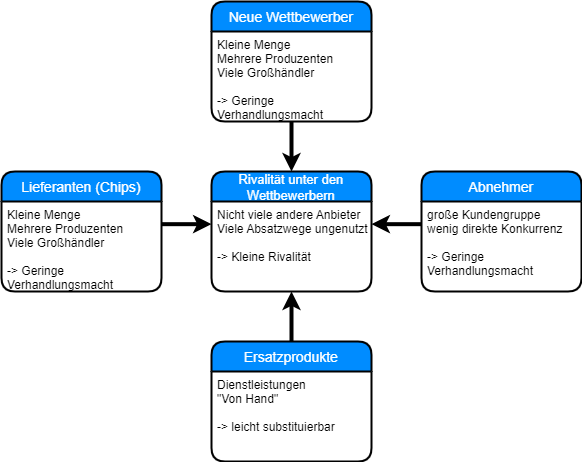
\includegraphics[width = 0.9\textwidth]{Eigene Darstellungen/Distributionswege2.png}

        \caption{Five Forces (Eigene Darstellung, in Anlehnung an \cite{Gamayanto2005}, S.\,127)}
    \end{figure}



\subsection{Marketingziele}
    Marketingziele werden formuliert, um die Ressourcen in einem Betreib gemeinsam in eine Richtung einzusetzen. Dabei
    geben die Ziele bei Entscheidungen eine Orientierung und sollen die Mitarbeiter motivieren. Die Ziele müssen
    erreichbar sein, damit die Mitarbeiter nicht demotiviert werden. Ein wichtiger Aspekt der Ziele ist die
    anschließende Kontrolle der Zielerfüllung und Abweichungsanalyse, um ggf. neue Maßnahmen ableiten zu können. Diese
    Ziele sind mittel- bis langfristig ausgelegt. (Vgl. \cite{Becker2018}, S.\,60)

    \noindent
    Um die unterschiedlichen Aspekte und Vorgaben der Zielsetzung zu berücksichtigen kann die SMART-Methode angewandt
    werden Die SMART-Methode geht auf Peter Drucker zurück und bietet Kriterien zur eindeutigen Formulierung von
    überprüfbaren und umsetzbaren Zielen. Jeder Buchstabe von SMART beinhaltet ein Kriterium an die Zielformulierung.
    Werden alle Kriterien eingehalten, können Unternehmensziele formuliert werden. (Vgl. \cite{Lawlor2012}, S.\,269)

    \begin{itemize}
        \item Spezifisch
        
            Das Ziel muss eindeutig und konkret formuliert sein. Es dürfen keine Missverständnisse entstehen. Bsp.: 
            \as Der Umsatz ist in diesem Jahr gegenüber dem Vorjahr zu steigern.\ad

        \item Messbar

            Die Erreichung des Ziels muss messbar sein. So werden quantitative und qualitative Anforderungen an das Ziel
            gesetzt. Eine objektive Bewertung muss möglich sein. Bsp.: \as Der Umsatz ist in diesem Jahr gegenüber dem
            Vorjahr um 15\% zu steigern.\ad

        \item Attraktiv
        
            Die Zielsetzung muss für die Teammitglieder attraktiv und akzeptabel sein. Können die Mitglieder sich nicht
            mit dem Ziel identifizieren so sinkt die Motivation. So sollte z.B. eine gemeinnützige Unternehmung keine
            moralisch verwerflichen Ziele anstreben. 

        \item Realistisch
        
            Das Ziel muss realistisch und damit umsetzbar formuliert sein. Ist die Erreichung des Ziels unrealistisch
            sinkt die Motivation das Ziel zu erreichen. Werden Zwischenziele erreicht kann das die Motivation weiter
            antreiben.

        \item Terminiert
        
            Um das Erreichen der Ziele kontrollieren zu können muss ein Zeitpunkt zur Zielerfüllung festgelegt sein.
            Folglich ist das Ziel in einer bestimmten Zeit zu erreichen. Nachdem die Zeit abgelaufen ist, kann die
            Kontrolle und Abweichungsanalyse starten.
    \end{itemize}


    %TODO Section machen

    \noindent
    Die Marketingziele für den RinnenRobo

    \begin{enumerate}
        \item Ziel
        
            Der RinnenRobo soll innerhalb eines Jahres 25\% Bekanntheit auf dem deutschen Fachmarkt erreicht haben.

        \item Ziel
        
            Nach drei Jahren sollen 10.000 Einheiten auf dem deutschen Massenmarkt (Privat- und Geschäftskunden)
            abgesetzt worden sein.

        \item Ziel
        
            Auf dem europäischen Markt soll eine Bekanntheit von ca. 5\% erreicht werden. Das bedeutet jeder zwanzigste
            Europäer soll Berührungspunkte mit unserem Produkt gesammelt haben. Dazu zählt auch Werbung.
    \end{enumerate}


\subsection{Distributionspolitik} \label{distro}
    Distribution beschreibt die betriebliche Funktion zwischen Hersteller und Verbraucher. Damit beschreibt die
    Distributionspolitik alle Entscheidungen und Maßnahmen auf dem Weg vom Anbieter zum Konsumenten.

    \noindent
    Die Distributionspolitik ist ein maßgebendes Instrument wie an den Kunden herangetreten wird. Die
    Distributionsentscheidungen sind im Regelfall langfristig ausgelegt. Es müssen je nach Produkt komplexe
    Distributionsketten auf- und ausgebaut werden.

    \noindent
    Die Distributionspolitik verfolgt dabei Ökonomische-, Versorgungs- und Psychologische Ziele. Hauptbestandteil der
    Ökonomischen Ziele ist der Erhalt und Ausbau des Betriebs in dem z.B. neue Kundengruppen erschlossen werden. Die
    Versorgungsziele beschäftigen sich unter anderem mit Lieferzuverlässigkeit und Liefergeschwindigkeit. Der dritte
    Bereich, die Psychologischen Ziele beinhalten insbesondere das Auftreten und die Wahrnehmung des Unternehmens.
    (Vgl. \cite{Bruhn2014}, S.\,245-278)

    \noindent
    Distributionswege lassen sich in zwei Arten unterscheiden, den direkten Vertrieb und den indirekten Vertrieb. Bei
    dem direkten Vertrieb übernehmen die Produzenten allein die Gestaltung des Verkaufsprozesses. Das Produkt oder die
    Dienstleistung wird ohne Zwischenhandel an den Konsumenten weitergegeben, z.B. Werksverkauf. Der indirekte Vertrieb
    verzichtet auf einen großen Teil der Distributionsaufgaben und liefert an einen Groß- oder Einzelhändler. Das
    Produkt wird nun entweder vom Händler direkt an den Kunden weitergegeben oder an einen weiteren Händler verkauft.

    \noindent
    Je nach Produkt und Kundengruppe reicht ein Distributionsweg nicht aus, um alle Kunden erreichen zu können. So
    können Unternehmen mit der Mehrwegdistribution über mehrere Absatzwege zeitgleich ihre Kunden erreichen. Eine solche
    Mehrwegdistribution ist mit einem erhöhten Koordinations- und Managementaufwand verbunden ermöglicht es aber
    Unternehmen das Marktpotenzial besser auszuschöpfen und Risiken auszugleichen.

    \noindent
    Auf den verschiedenen Wegen zum Konsumenten werden verschiedene Distributionsorgane angesprochen. Bei einer direkten
    Distribution werden insbesondere unternehmenseigene Distributionsorgane angesprochen. Der indirekte Vertrieb nutzt
    unternehmensfremde Distributionsorgane wie Absatzhelfer (z.B. Spedition) und Absatzmittler (Groß- und Einzelhandel).

    \noindent
    Die Breite der Distributionswegen entscheidet darüber, ob es sich um eine intensive (Universalvertrieb), eine
    selektive (ausgewählte Absatzmittler) oder eine exklusive Distribution (wenige, regulierte Anbieter) handelt.

    \noindent
    Der RinnenRobo soll über eine Mehrwegdistribution unterschiedliche Kundengruppen ansprechen und somit das
    Marktpotenzial bestmöglich nutzen (Siehe folgende Graphik). Per Online-Shop können die Kunden im direkten Vertrieb
    angesprochen werden. Weiter können im B2B Direktvertrieb und auf Messen Unternehmen die als Kunden agieren
    angesprochen werden. Weitere Kunden, wie z.B. den Eigenheimbesitzer können über den indirekten Vertrieb im Baumarkt
    erreicht werden. Die Wahl der Distributionswege lässt auf eine selektive Distribution schließen, welche sich
    besonders durch die Auswahl der Vertriebswege und Anforderungskriterien kennzeichnet. Ein solches Produkt bedarf
    zwar einer gewissen Expertise aber keiner Exklusivität.

     \begin{figure}[ht]
        \centering
        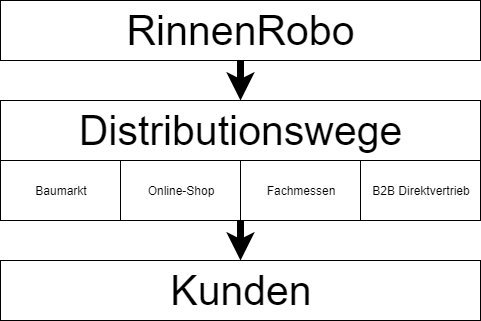
\includegraphics[width = 0.9\textwidth]{Eigene Darstellungen/Distributionswege1.png}

        \caption{Distributionswege (Eigene Dastellung in Anlehnung an Volesungsunterlagen)}
     \end{figure}
\pagebreak

% Verzeichnisse am Ende, erst das Glossar
\addonchapter{Zuordnung der Texte zu den Verfassern} % Es soll auch Glossar heißen
\begin{description}
\item[Persona A:] Jan Budde
\item[Persona B:] Jan Budde
\item[Branchenanalyse:] Jens Kessen 
\item[Konkurrenz-Analyse] Jens Kessen, Timon Menke, Jameel Hassan, Jan Budde 
\item[PEST-Analyse:] Jan Budde
\item[SWOT-Analyse:] Timon Menke
\item[Marketingziele:] Jens Kessen
\item[Produktpolitik:] Jameel Hassan
\item[Kommunikationspolitik:] Timon Menke
\item[Preispolitik:] Jan Budde
\item[Distributionspolitik:] Jens Kessen      
\end{description}

\pagebreak

% Literatur
\bibliographystyle{alphadin}									% Alphadin-Bibitem-Style zur Darstellung der Zitatkeys nach BA-Vorgabe
\renewcommand{\bibname}{Literatur}	%das literaturverzeichnis heißt ,,Literatur''
%\bibliography{literaturverzeichnis}
\bibliography{literaturverzeichnis}
% in JabRef bei Autorennamen Umlaute so schreiben: ö = {\"{o}}
\end{document}
